% !TEX root=./../main.tex
\section{Tutorial}
Рассказывались ВФ свободной частицы.
Это было в курсе квантмеха, поэтому кратко: 
\begin{align}
    \label{eq:psi_free-main-results}
    \nonumber
    E_n &= \frac{2\pi^2n^2}{L^2} & \psi_0 (x) &= \frac{1}{\sqrt{L}} \\
    \psi_n^\text{anti} (x) &= \sqrt{\frac{2}{L}} \sin \left( 2n \pi \frac{x}{L}\, \right) & \psi_n^{\text{symm}} (x) &= \sqrt{\frac{2}{L}\,} \cos \left( 2n\pi \frac{x}{L}\, \right)
\end{align}

Посмотреть в питоне на это можно в листинге \ref{code:free-periodic-sine-cosine}.
\pythonfile{programs_tutorial_5/free_periodic_sine_cosine}{Подсчет ВФ свободной частицы (\texttt{free\_periodic\_sine\_cosi.py})}{code:free-periodic-sine-cosine}

Все это дело в \eqref{eq:psi_free-main-results} можно выразить через комплексную экспоненту, что сделано в листинге \ref{code:free-periodic-complex-exp}.
\pythonfile{programs_tutorial_5/free_periodic_complex_exp}{Подсчет ВФ свободной частицы через комплексную экспоненту (\texttt{free\_periodic\_complex\_exp.py}}{code:free-periodic-complex-exp}

\begin{wrapfigure}{r}{0.3\linewidth}
    \label{fig:periodic-path}
    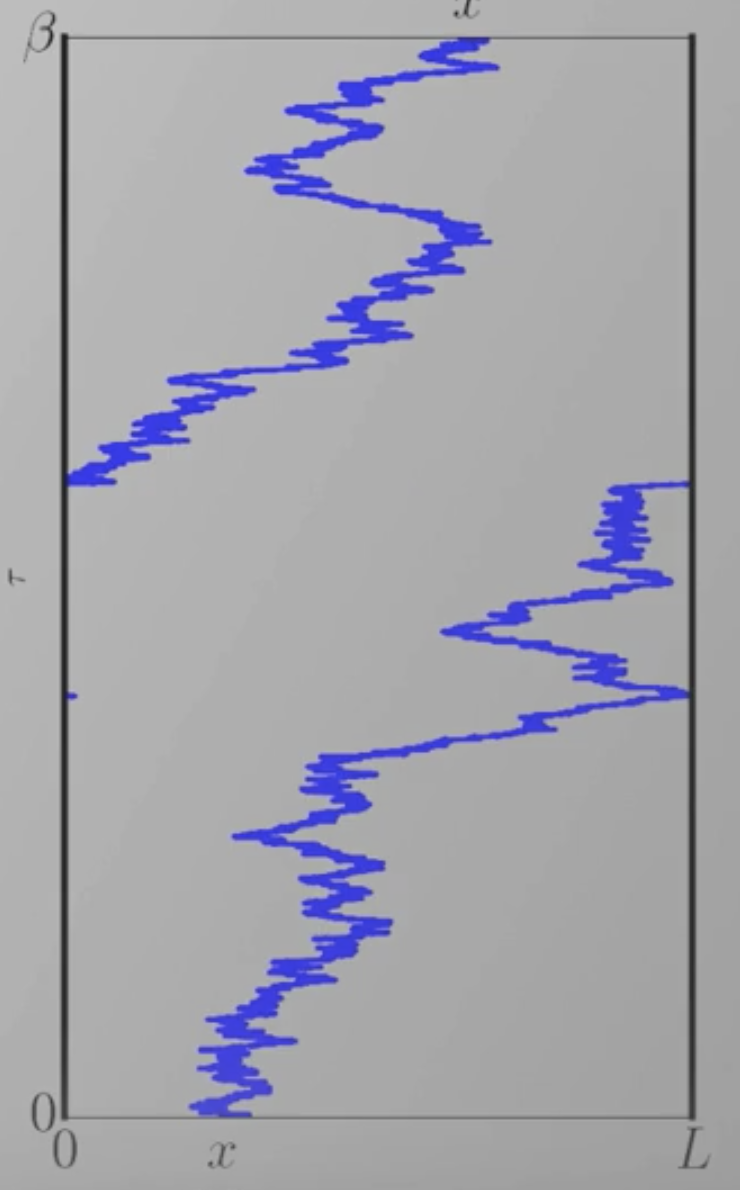
\includegraphics[width=\linewidth]{fig/periodic-path}
    \caption{Пример периодического пути с одним переходом через границу}
\end{wrapfigure}

Для периодических граничных условий $\rho$ имеет вид:
\begin{equation}
    \label{eq:rho-periodic-boundary-definition}
    \rho^{\text{per}} (x, x', \beta) = \sum\limits_{w=-\infty}^{+\infty}\rho^{\text{free}} (x, x' + wL, \beta)
\end{equation}

В tutorial рассказывали вывод Trotter approximation.
Там несложно, лучше посмотреть.

\subsection{Временная эволюция}
В большинстве своем, система эволюцинирует во времени. Надо это научиться считать.

Подход через УШ предполагает решение дифференциального уравнения с начальным условием $\psi (0) = \psi_0$. Решение можно записать через \textit{оператор эволюции}:
\begin{align}
    \label{eq:shroninger-equation_time-dependent}
    & i \frac{\partial}{\partial t}\, \psi (t) = \hat{H} \psi (t) & \Rightarrow &
    & \psi (t) = \exp(-it\hat{H}) \psi_0
\end{align}

Заменой $\beta = it$ (мнимое время) приводим $\exp(-it\hat{H}) = \exp(-\beta \hat{H})$, что есть оператор матрицы плотности:
\begin{equation}
    \label{eq:rho-via-hamiltonian}
    \hat{\rho} = \exp(-\beta \hat{H})
\end{equation}

Рассмотрим одномерную частицу в потенциале $V(x)$ с массой $m=1$.
Ее эволюция подчиняется УШ с гамильтонианом $\hat{H} = \hat{H}^{\text{free}} + \hat{V}(x)$.

Разобьем время на $N$ шагов $\Delta t = t / N$.
Получим, что
\begin{equation}
    \label{eq:evolution-operator-delta-t}
    \exp(-it\hat{H}) = \prod_{k=1}^N \exp(-i\Delta t \hat{H})
\end{equation}
\begin{equation}
    \label{eq:evolution-operator-delta-t-trotter}
    \exp(-i\Delta t [\hat{H}^{\text{free}} + V]) \approx
    {\color{blue} \exp\left( -i \frac{\Delta t}{2}\,\hat{V} \right)}
    {\color{red} \exp(-i\Delta t \hat{H}^{\text{free}})} 
    {\color{blue} \exp\left( -i \frac{\Delta t}{2}\,\hat{V} \right)}
    + O(\Delta t^3)
\end{equation}
Синим выделено то, что выполняется в прямом пространстве, красным --- в обратном (см. ниже).

В Фурье-пространстве действие $\hat{H}^{\text{free}}$ задается просто:
\begin{equation}
    \label{eq:evolution-free_fourier-space}
    \exp(-i \Delta t \hat{H}^{\text{free}}) \tilde \psi (p, t) = \underbrace{\exp\left( -i \Delta t \frac{p^2}{2}\, \right)}_\text{гауссиана} \tilde \psi (p, t) 
\end{equation}

Это дает алгоритм (листинг \ref{code:quantum_time_evolution}):
\begin{enumerate}
    \item Умножаем на $\exp(-i \frac{\Delta t}{2}\,V)$ значение $\psi(x)$.
    \item Переводим результат в Фурье-пространство (см. смену цветов в \eqref{eq:evolution-operator-delta-t-trotter}).
    \item Действуем по правилу \eqref{eq:evolution-free_fourier-space} на $\psi(p)$.
    \item Возвращаемся в прямое пространство.
    \item Умножаем на $\exp(-i \frac{\Delta t}{2}\,V)$ значение $\psi(x)$.
\end{enumerate}
Порядок действий нельзя переставлять, так как имеем дело с операторами.

\pythonfile{programs_tutorial_5/quantum_time_evolution}{Эволюция во времени для квантовой частицы (\texttt{quantum\_time\_evolution.py})}{code:quantum_time_evolution}

Посмотрите на эти графики, они правда красивые!
